\documentclass[12pt,a4paper]{article}
\usepackage[a4paper,margin=1in]{geometry}
\usepackage{graphicx}
\usepackage{booktabs}
\usepackage{amsmath,amssymb}
\usepackage{float}
\usepackage{hyperref}
\usepackage{xcolor}
\usepackage{listings}
\usepackage{enumitem}
\usepackage{fancyhdr}
\usepackage{longtable}
\hypersetup{colorlinks=true,linkcolor=blue,urlcolor=blue}
\pagestyle{fancy}
\fancyhf{}
\lhead{ICS1512}
\rhead{Machine Learning Algorithms Laboratory}
\cfoot{\thepage}
\lstset{
language=Python,
basicstyle=\ttfamily\small,
numbers=left,
frame=single,
breaklines=true,
showstringspaces=false
}
\begin{document}
\begin{tabular}{|p{4cm}|p{11cm}|}
\hline
Experiment No. & 3\\ \hline
Experiment Title & Regression Analysis using Linear and Regularized Models (Loan Amount Prediction)\\ \hline
GitHub Repository & \url{https://github.com/Dharika-2006/ML-LAB-ASSIGMENTS} \\ \hline
Student Name & Dharika Shree K\\ \hline
Register Number & 3122247001014\\ \hline
Faculty & Dr. Poreddy Ajay Kumar Reddy \\ \hline
Submission Date & 02.08.26\\ \hline
\end{tabular}
\section{Objective}

To implement and compare Linear Regression, Ridge Regression, Lasso Regression, and Elastic Net Regression for predicting loan amounts. The experiment involves performing exploratory data analysis, handling missing values, encoding categorical features, scaling numerical features, tuning hyperparameters using GridSearchCV, and evaluating model performance using MAE, MSE, RMSE, R\textsuperscript{2}-score, learning curves, and training time.

\section{Problem Statement}

\textbf{Problem:} To build and compare different regression models on the Loan Amount Prediction dataset in order to estimate the loan amount sanctioned to an applicant and analyze the effect of regularization on model performance.

\textbf{Input:} Unclean Loan Amount Prediction dataset.

\textbf{Output:} A cleaned and preprocessed dataset, exploratory data analysis, trained Linear Regression, Ridge Regression, Lasso Regression, and Elastic Net models, optimized hyperparameters, prediction and residual plots, learning curves, coefficient comparison, and performance metrics including MAE, MSE, RMSE, and R\textsuperscript{2}-score.

\section{Dataset Description}

\begin{longtable}{|p{6cm}|p{8cm}|}
\hline
Dataset Name & Loan Amount Prediction (uncleaned) dataset\\ \hline
Dataset Source & Kaggle\\ \hline
Number of Samples & 650\\ \hline
Number of Features & 21\\ \hline
Number of Classes & This is a regression problem, so the target variable is continuous rather than belonging to fixed classes.\\ \hline
Missing Values & 209\\ \hline
Train-Test Split & 80\% training, 20\% testing\\ \hline
\end{longtable}

\section{Exploratory Data Analysis}

\begin{itemize}
\item Dataset overview
\item Statistical summary
\item Missing value analysis
\item Target distribution
\item Correlation analysis
\item Feature distribution
\end{itemize}

\subsection*{Figure: Loan Amount Distribution}
\begin{figure}[H]
\centering
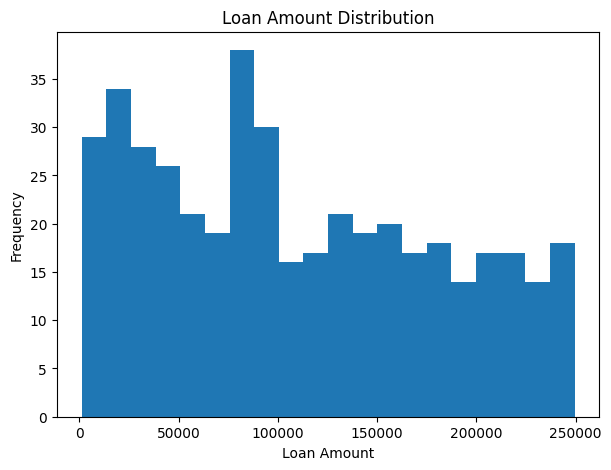
\includegraphics[width=0.7\linewidth]{hist`.png}
\caption{Histogram of the target variable \texttt{loan\_amount}}
\end{figure}

\textbf{Inference:}

The histogram shows that the loan amounts are spread across a wide range, from approximately 1,143 to 249,584, with an average value of around 109,489. Instead of being concentrated around a single value, the data is distributed over a broad interval, indicating high variability in the target. Because of this large variation, predicting loan amounts becomes more challenging, and naturally larger error values such as MSE and RMSE can be expected. Therefore, the R\textsuperscript{2}-score is also an important metric, as it indicates how much of this variation is explained by the regression model.

\subsection*{Figure: Feature vs Loan Amount Scatter Plots}
\begin{figure}[H]
\centering
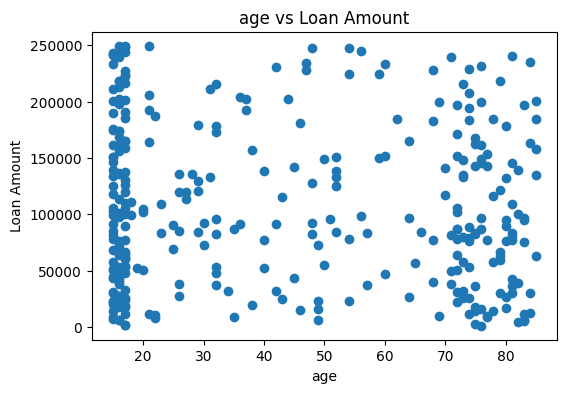
\includegraphics[width=0.4\linewidth]{scatter1.png}
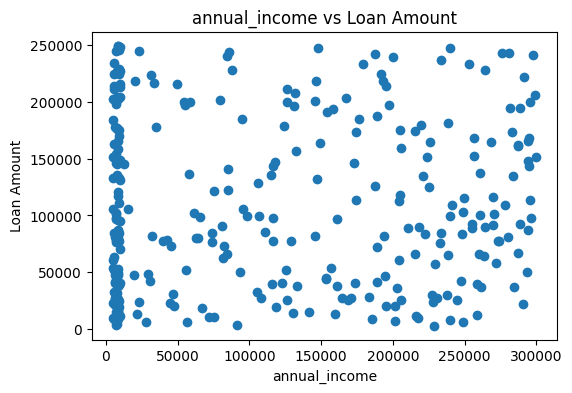
\includegraphics[width=0.4\linewidth]{scatter2.png}
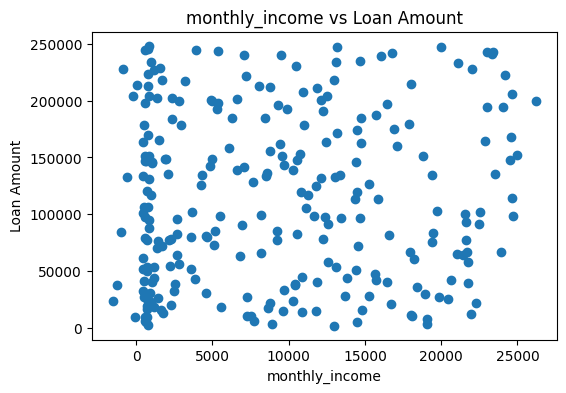
\includegraphics[width=0.4\linewidth]{scatter3.png}
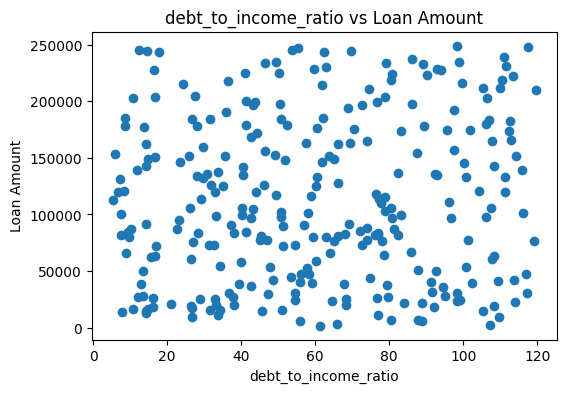
\includegraphics[width=0.4\linewidth]{scatter4.png}
\caption{Scatter plots of \texttt{age}, \texttt{annual\_income}, \texttt{monthly\_income}, and \texttt{debt\_to\_income\_ratio} against \texttt{loan\_amount}}
\end{figure}

\textbf{Inference:}

The scatter plots do not show a clear linear relationship between any individual feature and the loan amount. Most points are widely scattered, indicating that no single feature alone has a strong influence on the target variable. This observation matches the relatively low R\textsuperscript{2} values obtained during model evaluation. It also suggests that the prediction depends on the combined effect of several features rather than any one feature by itself.

\subsection*{Figure: Statistical Summary and Missing Values}
\begin{figure}[H]
\centering
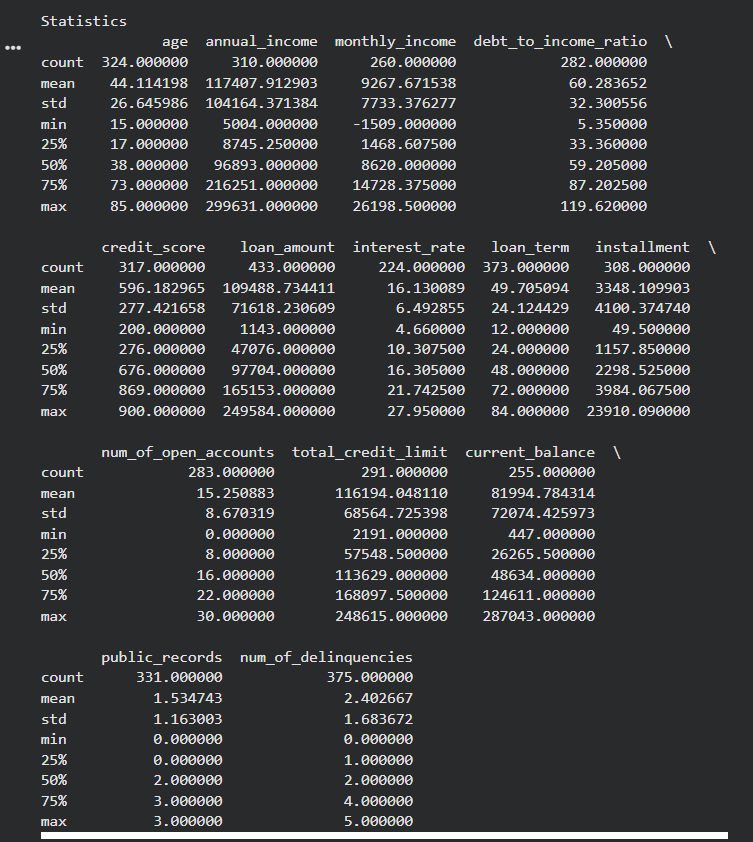
\includegraphics[width=0.4\linewidth]{summ1.png}
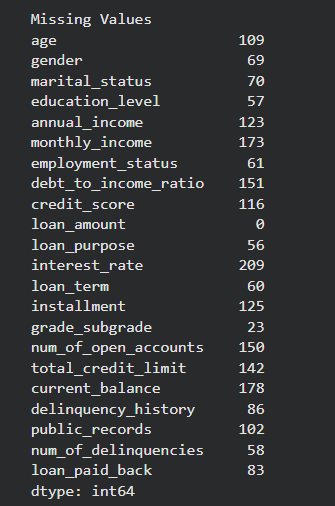
\includegraphics[width=0.4\linewidth]{miss1.png}
\caption{Descriptive statistics and missing-value counts per column}
\end{figure}

\textbf{Inference:}

The statistical summary and missing-value analysis show that several features contain a large number of missing entries. Columns such as \texttt{interest\_rate}, \texttt{current\_balance}, and \texttt{monthly\_income} have a considerable amount of missing data, making preprocessing an essential step before training the models. Median imputation for numerical features and mode imputation for categorical features helped retain the available data instead of removing a large number of records. However, extensive missing values may still reduce the predictive quality of the final models.

\subsection*{Figure: Class Distribution}

\textbf{Inference:}

Since this is a regression problem, the target variable is continuous and there are no class labels. Therefore, a class distribution plot is not applicable. The histogram of the loan amount serves the same purpose by illustrating how the target values are distributed across the dataset.

\subsection*{Figure: Correlation Matrix}

\begin{figure}[H]
\centering

\includegraphics[width=1\linewidth]{corr1.png}
\caption{Correlation among numeric features and coefficient trends}
\end{figure}

\textbf{Inference:}

The coefficient comparison indicates that features such as \texttt{installment}, \texttt{loan\_term}, and \texttt{public\_records} contribute more strongly to predicting the loan amount than the remaining features. Some variables, including \texttt{credit\_score} and \texttt{interest\_rate}, show changes in coefficient signs across different regression models, suggesting that their relationship with the target is relatively weak and may also be affected by multicollinearity.

\subsection*{Feature Distribution}

The numerical features in the dataset have very different value ranges. For example, \texttt{age} is measured in tens, whereas \texttt{annual\_income} is measured in thousands. To ensure that all features contribute equally during model training, standardization was applied using \texttt{StandardScaler}. The categorical features also contain inconsistent labels, such as different capitalizations of the same category, which indicates that additional data cleaning could further improve the quality of the dataset before model training.

\section{Data Preprocessing}
\begin{itemize}
\item \textbf{Missing value handling:} Rows with a missing target (\texttt{loan\_amount}) were dropped first, reducing the dataset from 650 to 433 rows. For the remaining features, a \texttt{ColumnTransformer} routed numeric columns through a \texttt{SimpleImputer(strategy="median")} and categorical columns through a \texttt{SimpleImputer(strategy="most\_frequent")}, so that missing numeric values were filled with the column median and missing categorical values with the most frequent category.
\item \textbf{Encoding:} All categorical features were encoded using \texttt{OneHotEncoder(handle\_unknown="ignore")}, converting each category into a binary indicator column and safely ignoring any unseen category at prediction time.
\item \textbf{Feature scaling:} All numeric features were standardized using \texttt{StandardScaler} (zero mean, unit variance), which is essential for Ridge, Lasso and Elastic Net since their regularization penalties are scale-sensitive.
\item \textbf{Train-test split:} The cleaned dataset (433 rows) was split into 80\% training and 20\% testing sets using \texttt{train\_test\_split} with \texttt{test\_size=0.20} and \texttt{random\_state=42}.
\item \textbf{Feature engineering:} No new engineered features were created; the pipeline used the 13 numeric and 8 categorical columns as provided (after imputation, scaling, and one-hot encoding), combined via a single \texttt{ColumnTransformer} inside a \texttt{Pipeline} together with each regression model.
\end{itemize}

\section{Machine Learning Algorithm}
\subsection*{Linear Regression}
\textbf{Working principle:} Fits a linear relationship between the input features and the continuous target by minimizing the sum of squared residuals.

\textbf{Mathematical formulation:}
\[
\hat{y} = \beta_0 + \sum_{i=1}^{n}\beta_i x_i, \qquad
\min_{\beta}\ \sum_{j=1}^{m}\left(y_j - \hat{y}_j\right)^2
\]

\textbf{Advantages:} Simple, interpretable coefficients, computationally cheap, no hyperparameters to tune.

\textbf{Limitations:} Prone to overfitting with many correlated/noisy features, sensitive to multicollinearity, assumes a linear relationship and can perform poorly (even negative R\textsuperscript{2}) when this assumption does not hold, as observed in this experiment.

\subsection*{Ridge Regression (L2 Regularization)}
\textbf{Working principle:} Adds an L2 penalty on the coefficient magnitudes to shrink them towards zero, reducing variance and multicollinearity sensitivity at the cost of a small bias.

\textbf{Mathematical formulation:}
\[
\min_{\beta}\ \sum_{j=1}^{m}\left(y_j - \hat{y}_j\right)^2 + \alpha \sum_{i=1}^{n}\beta_i^2
\]

\textbf{Advantages:} Handles multicollinearity well, more stable coefficient estimates than plain Linear Regression, retains all features.

\textbf{Limitations:} Does not perform feature selection (coefficients shrink but rarely reach exactly zero), requires tuning $\alpha$.

\subsection*{Lasso Regression (L1 Regularization)}
\textbf{Working principle:} Adds an L1 penalty on the coefficient magnitudes, which can shrink some coefficients exactly to zero, effectively performing automatic feature selection.

\textbf{Mathematical formulation:}
\[
\min_{\beta}\ \sum_{j=1}^{m}\left(y_j - \hat{y}_j\right)^2 + \alpha \sum_{i=1}^{n}|\beta_i|
\]

\textbf{Advantages:} Produces sparse, more interpretable models by zeroing out unimportant features (e.g.\ \texttt{cat\_\_gender\_Female} was reduced exactly to 0 in this experiment).

\textbf{Limitations:} Can be unstable when features are highly correlated (may arbitrarily pick one of several correlated features), needs a higher \texttt{max\_iter} to converge, and requires tuning $\alpha$.

\subsection*{Elastic Net}
\textbf{Working principle:} Combines both L1 and L2 penalties, controlled by a mixing parameter $l1\_ratio$, balancing feature selection (Lasso-like behaviour) with coefficient shrinkage/stability (Ridge-like behaviour).

\textbf{Mathematical formulation:}
\[
\min_{\beta}\ \sum_{j=1}^{m}\left(y_j - \hat{y}_j\right)^2 + \alpha\left(l1\_ratio\sum_{i=1}^n|\beta_i| + \frac{1-l1\_ratio}{2}\sum_{i=1}^n \beta_i^2\right)
\]

\textbf{Advantages:} More flexible than pure Ridge or Lasso, performs well when features are correlated, and achieved the best test R\textsuperscript{2} in this experiment.

\textbf{Limitations:} Two hyperparameters ($\alpha$ and $l1\_ratio$) to tune instead of one, higher computational cost, and results can still be sensitive to the quality of feature scaling/imputation.

\section{Experimental Setup}
\begin{tabular}{ll}
\toprule
Python Version & 3 (exact version not captured; run on Google Colab's Python 3 runtime)\\
Scikit-Learn Version & As installed in the Colab environment (verify with \texttt{sklearn.\_\_version\_\_})\\
IDE & Google Colaboratory (Jupyter-based notebook)\\
Operating System & Linux (Google Colab backend)\\
Hardware & Google Colab-provided CPU runtime (not explicitly specified in the notebook)\\
\bottomrule
\end{tabular}

\section{Hyperparameter Selection}
\begin{tabular}{ll}
\toprule
Parameter & Value\\
\midrule
Train-Test Split Ratio & 80 : 20\\
Random State & 42\\
Cross-Validation (GridSearchCV) & 5-fold, scoring = $R^2$\\
Linear Regression & No hyperparameters tuned (baseline model)\\
Ridge -- search space & $\alpha \in \{0.01, 0.1, 1, 10, 100\}$\\
Ridge -- best parameters & $\alpha = 100$ (Best CV $R^2$ = 0.0850)\\
Lasso -- search space & $\alpha \in \{0.001, 0.01, 0.1, 1, 10\}$ ($max\_iter=10000$)\\
Lasso -- best parameters & $\alpha = 10$ (Best CV $R^2$ = $-0.1282$)\\
Elastic Net -- search space & $\alpha \in \{0.01, 0.1, 1, 10\}$, $l1\_ratio \in \{0.2, 0.5, 0.8\}$ ($max\_iter=10000$)\\
Elastic Net -- best parameters & $\alpha = 1$, $l1\_ratio = 0.5$ (Best CV $R^2$ = 0.0860)\\
\bottomrule
\end{tabular}

\section{Results}
\begin{longtable}{lccccc}
\toprule
Model & MAE & MSE & RMSE & R\textsuperscript{2}-score & Training Time (s)\\
\midrule
Linear Regression & 54649.60 & $4.590\times10^{9}$ & 67747.34 & $-0.0454$ & 0.0907\\
Ridge Regression & 51150.94 & $3.927\times10^{9}$ & 62669.65 & 0.1054 & 0.6124\\
Lasso Regression & 54582.94 & $4.577\times10^{9}$ & 67652.01 & $-0.0424$ & 3.1482\\
Elastic Net & 51570.51 & $3.904\times10^{9}$ & 62479.82 & 0.1109 & 1.4580\\
\bottomrule
\end{longtable}
\noindent Elastic Net achieved the best test-set $R^2$ (0.1109) and one of the lowest RMSE values, closely followed by Ridge Regression (R\textsuperscript{2} = 0.1054). Plain Linear Regression and Lasso Regression both produced a \emph{negative} $R^2$ on the test set, meaning they performed worse than a model that simply predicts the mean loan amount for every applicant -- a clear sign of overfitting/instability in the unregularized (or under-regularized) linear model on this noisy, heavily-imputed dataset.

\section{Result Visualization}
Include all graphs generated during the experiment.

\subsection*{1. Correlation Matrix / Coefficient Comparison}
\begin{figure}[H]
\centering

\includegraphics[width=1\linewidth]{corr1.png}
\caption{Comparison of feature coefficients across Linear, Ridge, Lasso and Elastic Net models}
\end{figure}
\textbf{Inference:}
\texttt{installment} has by far the largest positive coefficient in every model (28,566 for Linear Regression down to 17,962 for Elastic Net), confirming it as the single strongest numeric predictor of loan amount. Regularization visibly shrinks large coefficients: \texttt{loan\_term}'s coefficient drops from 9,695 (Linear Regression) to 3,141 (Elastic Net), and \texttt{installment} similarly shrinks under stronger regularization, which is the expected behaviour of Ridge/Lasso/Elastic Net penalties. Lasso drove the \texttt{cat\_\_gender\_Female} coefficient exactly to zero, demonstrating its feature-selection property, while Elastic Net kept a small non-zero value for the same feature, reflecting its blended L1/L2 penalty. This comparison also reveals sign instability in weaker features such as \texttt{credit\_score} and \texttt{interest\_rate}, which further indicates these features have a weak or noisy relationship with the target once other features are accounted for.

\subsection*{2. Class Distribution}
\textbf{Not applicable} -- this is a regression task with a continuous target rather than discrete classes; refer to the Loan Amount Distribution histogram in Section~4 instead.

\subsection*{3. Confusion Matrix}
\textbf{Not applicable} -- confusion matrices are used for classification tasks. As a regression-appropriate substitute, the following Predicted-vs-Actual and Residual plots were generated for each model.

\begin{figure}[H]
\centering
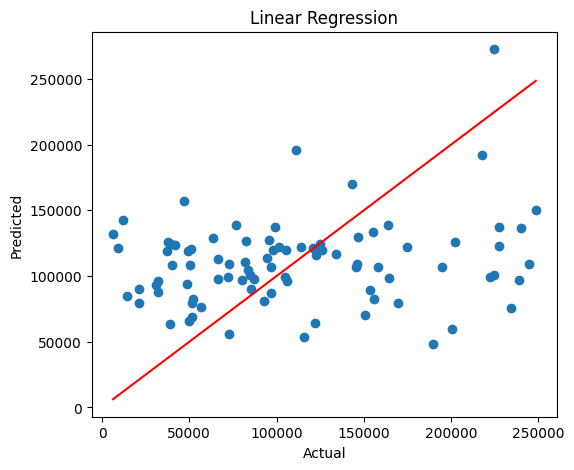
\includegraphics[width=0.4\linewidth]{actvspred.png}
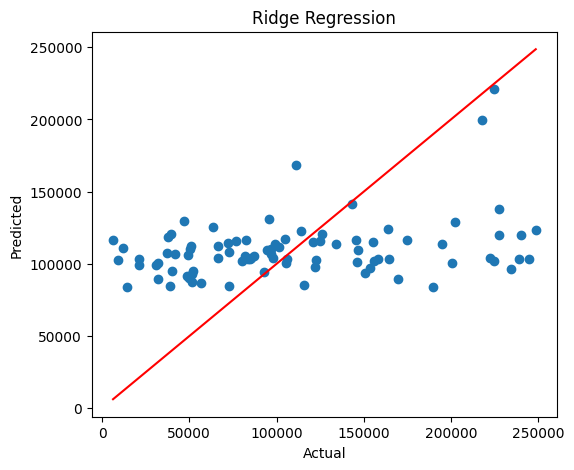
\includegraphics[width=0.4\linewidth]{act2.png}
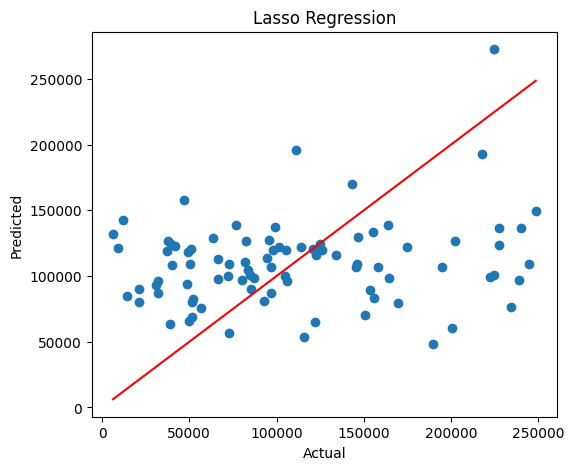
\includegraphics[width=0.4\linewidth]{act3.png}
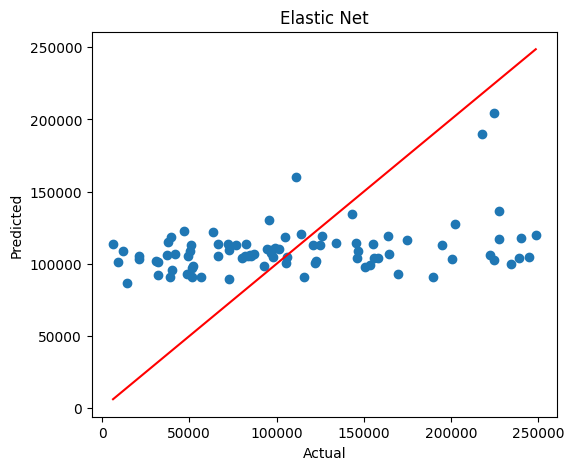
\includegraphics[width=0.4\linewidth]{act4.png}
\caption{Predicted vs.\ Actual loan amount for each of the four models}
\end{figure}
\textbf{Inference:}
For all four models, the predicted-vs-actual scatter points are widely dispersed around the ideal diagonal reference line rather than tightly hugging it, visually confirming the low $R^2$ scores (all below 0.12). Ridge and Elastic Net show slightly tighter clustering near the diagonal than Linear Regression and Lasso, consistent with their higher $R^2$ values. None of the models show a systematic bias toward over- or under-prediction across the whole range, but predictions are visibly compressed toward the middle of the loan-amount range compared to the true spread of actual values, a typical symptom of models that have not captured enough predictive signal from the available features.

\begin{figure}[H]
\centering
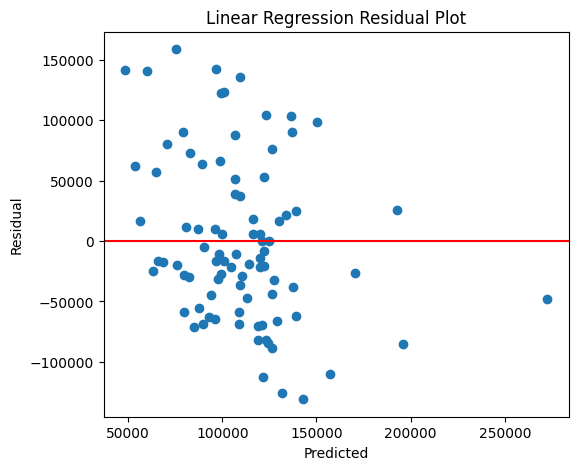
\includegraphics[width=0.4\linewidth]{res1.png}
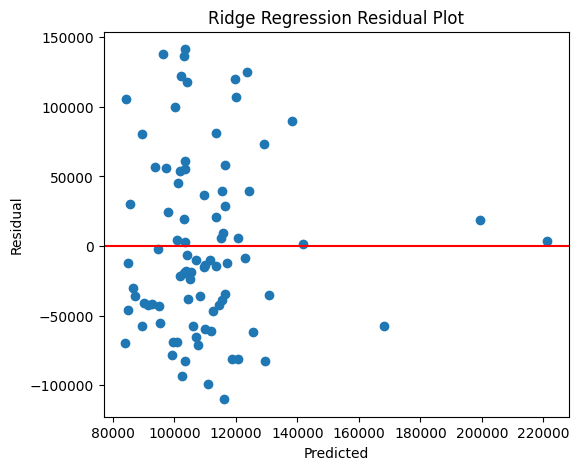
\includegraphics[width=0.4\linewidth]{res2.png}
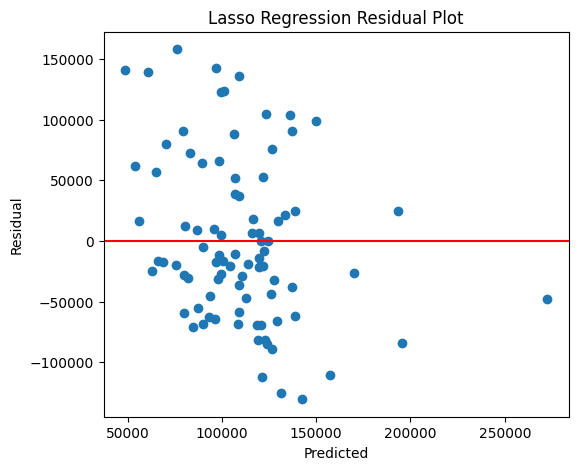
\includegraphics[width=0.4\linewidth]{res3.png}
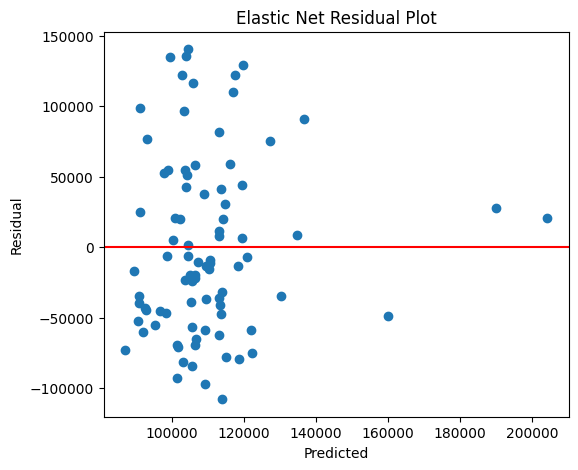
\includegraphics[width=0.4\linewidth]{res4.png}
\caption{Residual plots (Predicted vs.\ Residual) for each of the four models}
\end{figure}
\textbf{Inference:}
The residual plots show residuals scattered fairly randomly around the zero line without an obvious funnel (heteroscedasticity) or curved pattern, suggesting the models are not grossly misspecified in functional form. However, the residual spread is large relative to the target's own scale, again reflecting the low proportion of target variance explained. Ridge and Elastic Net show a marginally tighter residual band than Linear Regression and Lasso, consistent with their better R\textsuperscript{2} scores.

\subsection*{4. ROC Curve}
\textbf{Not applicable} -- ROC curves apply to binary/multi-class classification problems and do not apply to this continuous-target regression task.

\subsection*{5. Precision-Recall Curve}
\textbf{Not applicable} -- Precision-Recall curves likewise apply only to classification tasks and are not relevant to predicting a continuous loan amount.

\subsection*{6. Learning Curve}
\begin{figure}[H]
\centering
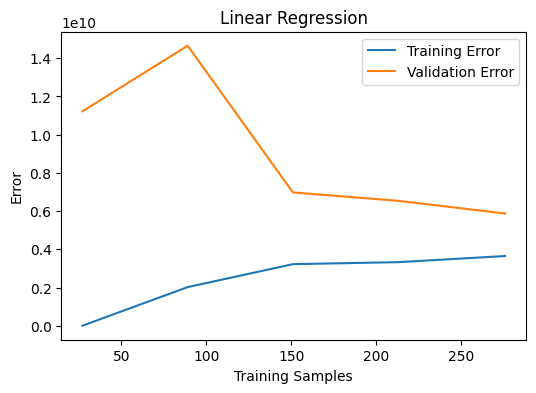
\includegraphics[width=0.4\linewidth]{val1.png}
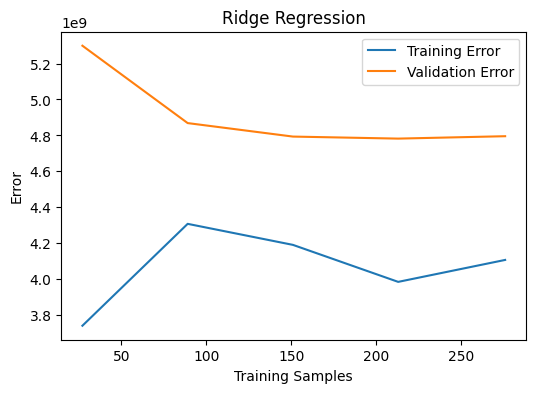
\includegraphics[width=0.4\linewidth]{val2.png}
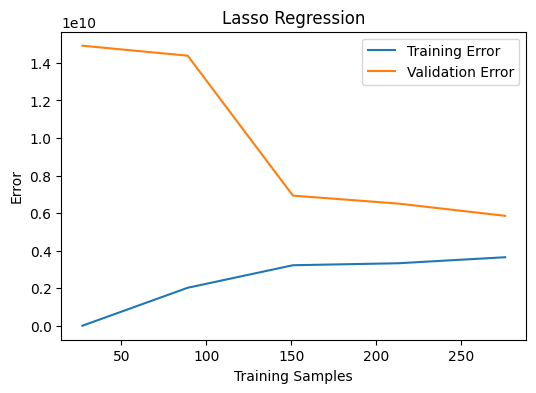
\includegraphics[width=0.4\linewidth]{val3.png}
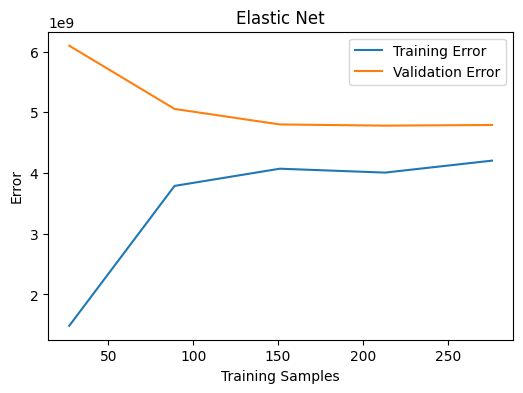
\includegraphics[width=0.4\linewidth]{val4.png}
\caption{Learning curves (Training Error vs.\ Validation Error) for each model}
\end{figure}
\textbf{Inference:}
The learning curves show that the training error remains lower than the validation error for all four models, indicating a gap between training and testing performance. Ridge and Elastic Net have a smaller gap than Linear Regression and Lasso, showing better generalization due to regularization. Since the curves do not converge even with more training samples, the results suggest that the limited data and high number of missing values had a greater impact on performance than the choice of regression model.


\subsection*{7. Feature Importance}
As shown in the Coefficient Comparison plot above, \texttt{installment}, \texttt{loan\_term}, and \texttt{public\_records} are the most influential numeric features across all four models, while several one-hot encoded categorical indicators (e.g., inconsistent \texttt{gender} categories) contribute comparatively small and unstable coefficients, suggesting limited predictive value and/or a need for better categorical cleaning prior to encoding.

\section{Discussion}
All four regression models showed relatively low predictive performance, with Elastic Net achieving the highest test R\textsuperscript{2}-score of 0.1109. Linear Regression and Lasso Regression produced negative R\textsuperscript{2} values, indicating that they were less effective on this dataset. One major reason is the large number of missing values, which required extensive imputation and reduced the amount of useful information available for learning.

Regularization improved the overall performance, with Ridge and Elastic Net giving better and more stable results than the baseline Linear Regression. The learning curves also suggest that the models were limited more by the quality of the dataset than by model complexity. Although the comparison was fair due to consistent preprocessing and 5-fold GridSearchCV, further improvements could be achieved through better data cleaning, feature engineering, and the use of more advanced non-linear models.


\section{Conclusion}
This experiment compared Linear Regression, Ridge Regression, Lasso Regression, and Elastic Net for loan amount prediction. The dataset was preprocessed using missing value imputation, one-hot encoding, feature scaling, an 80:20 train-test split, and 5-fold GridSearchCV for hyperparameter tuning.

Elastic Net ($\alpha = 1$, $l1\_ratio = 0.5$) achieved the best performance (R\textsuperscript{2} = 0.1109, RMSE $\approx$ 62,480), closely followed by Ridge Regression. The results show that regularization improves performance on noisy datasets, while better data quality and feature engineering could further enhance prediction accuracy.

\section{References}
\begin{enumerate}
\item Scikit-learn developers,Linear Models,scikit-learn documentation: \url{https://scikit-learn.org/stable/modules/linear_model.html}
\item Scikit-learn developers, sklearn.compose.ColumnTransformer,scikit-learn documentation: \url{https://scikit-learn.org/stable/modules/generated/sklearn.compose.ColumnTransformer.html}
\item Scikit-learn developers,sklearn.model\_selection.learning\_curve, scikit-learn documentation: \url{https://scikit-learn.org/stable/modules/generated/sklearn.model_selection.learning_curve.html}
\item Kaggle,Loan Amount Prediction (uncleaned) dataset,Kaggle Datasets: \url{https://www.kaggle.com/datasets}
\end{enumerate}
\end{document}